% LHCb VELO upgrade presentation for 23 March 2017
% Topic:    Isolation flagging module progress
% Author:   Dónal Murray
% Date:     21 March 2017

% $Header$
\documentclass{beamer}
\mode<presentation>
\usefonttheme{professionalfonts}
\setbeamertemplate{footline}[text line]{%
  \parbox{\linewidth}{\vspace*{-22pt}\tiny\insertshortauthor}}
\setbeamertemplate{navigation symbols}{} % remove beamer symbols

\usepackage[english]{babel}
\usepackage[utf8]{inputenc}
\usepackage{times}
\usepackage[T1]{fontenc}
\usepackage{pgf}

\title{SPP Isolation Flagging Module}
\subtitle{Progress Update}
\author[Dónal Murray\hspace*{80pt}donal.murray@cern.ch]{Dónal Murray \\
  \vskip7pt
  \tiny{donal.murray@cern.ch}
}
\institute{}
\date{23 March 2017}

\pgfdeclareimage[height=1.5cm]{university-logo}{UoMlogo}
\logo{\pgfuseimage{university-logo}}

% $Document$
\begin{document}

{
\setbeamertemplate{footline}{} % do not display footer on titlepage
\begin{frame}
  \titlepage
\end{frame}
}
\addtocounter{framenumber}{-1} % do not count titlepage in slide count

\begin{frame}{Overview}
  \tableofcontents
\end{frame}


% Structuring a talk is a difficult task and the following structure
% may not be suitable. Here are some rules that apply for this
% solution:

% - Exactly two or three sections (other than the summary).
% - At *most* three subsections per section.
% - Talk about 30s to 2min per frame. So there should be between about
%   15 and 30 frames, all told.

% - A conference audience is likely to know very little of what you
%   are going to talk about. So *simplify*!
% - In a 20min talk, getting the main ideas across is hard
%   enough. Leave out details, even if it means being less precise than
%   you think necessary.
% - If you omit details that are vital to the proof/implementation,
%   just say so once. Everybody will be happy with that.

\section{Concept}

\subsection{Function of the SPP isolation flagging module}

\begin{frame}{The SPP isolation flagging module}
  \begin{figure}
    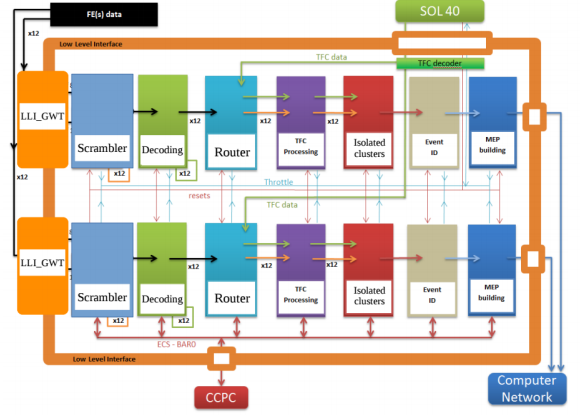
\includegraphics[scale=0.3]{Overview}
    \caption{\centering Drop in module (shown as "Isolated Clusters" in this image) to check for isolated clusters.}
  \end{figure}
\end{frame}


\begin{frame}{The event isolation flagging module}{Columns in the SPP}
  \begin{figure}
    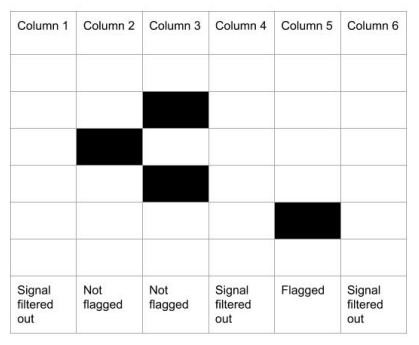
\includegraphics[scale=0.3]{Columns}
    \caption{\centering Columns with no neighbours are flagged. Doing this in the FPGA reduces load on CPU in software stage.}
  \end{figure}
\end{frame}

\subsection{Block Diagrams}

\begin{frame}{The event isolation flagging module}{Top level block Diagram}
  \begin{figure}
    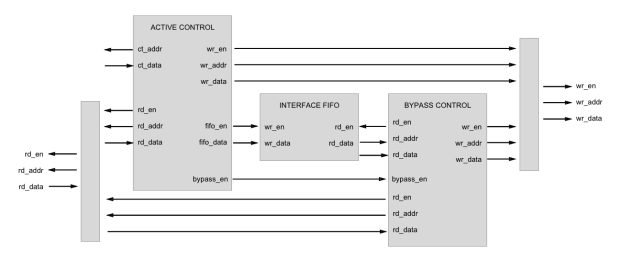
\includegraphics[scale=0.4]{TopLevelBlock}
  \end{figure}
  \begin{itemize}
    \item
      Checks each column in SPP to see if it is isolated.
  \end{itemize}
\end{frame}

\begin{frame}{Active Control}
  \begin{figure}
    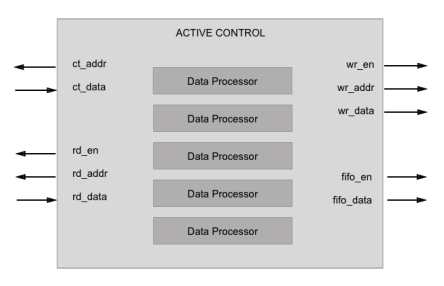
\includegraphics[scale=0.3]{ActiveControl}
  \end{figure}
  \begin{itemize}
    \item
      Assigns tasks to the next free data processor
    \item
      Keeps track of clock cycles.
  \end{itemize}
\end{frame}

\begin{frame}{Data Processor}
  \begin{figure}
    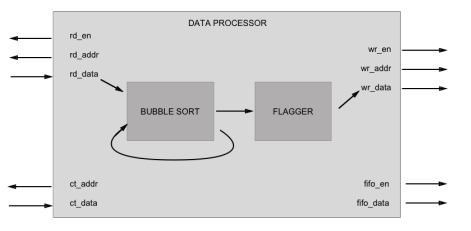
\includegraphics[scale=0.3]{DataProcessor}
  \end{figure}
  \begin{itemize}
    \item

    \item

  \end{itemize}
\end{frame}





\section{Implementation}

\subsection{Implementation in VHDL}

\begin{frame}{Implementation in VHDL}
  \begin{itemize}
    \item
      Using code started by masters students last year
    \item
      Code now compiles and can be simulated in Modelsim.
    \end{itemize}
\end{frame}


\subsection{Testing in Modelsim}

\begin{frame}{Testing in Modelsim}
  \begin{itemize}
    \item
      All low level blocks tested and working
    \item
      Generated random data packages to test at top level
    \item
      Next step: test with realistic data.
  \end{itemize}
\end{frame}


\subsection{Incorporation into the full AMC40 Firmware}

\begin{frame}{Incorporation into the full AMC40 Firmware}
  \begin{itemize}
    \item
      Cloned the full AMC40 firmware repository (velo24 branch)
    \item
      Inserted data processing block
    \item
      Next step: ... .
  \end{itemize}
\end{frame}



\section*{Summary}

\begin{frame}{Summary}

  % Keep the summary as short as possible
  \begin{itemize}
  \item
    Implementation in Modelsim is complete; mid way through testing
  \item

  \end{itemize}

  % Next steps
  \vskip0pt plus.5fill
  \begin{itemize}
  \item
    Outlook
    \begin{itemize}
    \item
      Complete testing in Modelsim with realistic data
    \item
      Test as a standalone module in Quartus
    \item
      Incorporate into full AMC40 firmware.
    \end{itemize}
  \end{itemize}
\end{frame}

\end{document}
